% !TeX spellcheck = en_GB
% !TeX encoding = UTF-8
\documentclass[8pt]{beamer}

\usepackage[utf8]{inputenc}                                                     
 \usetheme[block=fill,progressbar=foot,background=light]{metropolis}                                                               
%  \usecolortheme{crane}                                                       
  %\useinnertheme{circles}                                                         
  \usepackage[english]{babel}                                                     
  \usepackage{csquotes}                                                           
  \usepackage[T1]{fontenc}                                                        
  \usepackage{booktabs}                                                       \usepackage{pgfgantt}
  \usepackage{pifont}
  \usepackage{adfbullets}
  \usepackage{enumitem}
  \usepackage{amsmath}   
  \usepackage{tikz}
  \usepackage{amssymb}
  \usepackage{amsfonts}
  \usepackage{mathrsfs}   
  \usepackage{graphicx}
  \usepackage{adjustbox}
  \usepackage{varioref}
  \usepackage{probsoln}
  \usepackage{attachfile2}
  \usepackage{pgfplots}
\pgfplotsset{compat=newest}
  \usepackage[style=authoryear,backref=true]{biblatex}
 \usepackage[]{hyperref} 
  \graphicspath{{Graphics/}}
  \usepackage{multirow,array}
  \addbibresource{../Everything.bib}
  \usepackage{colortbl}
  \definecolor{aa}{RGB}{255, 124, 0}
  \definecolor{cc}{RGB}{230, 230, 230}    
  %\setbeamercolor{palette tertiary}{fg=aa,bg=cc}
  %\setbeamercolor{structure}{fg=cc}
  %\setbeamercolor{alerted text}{fg=red}
  
  %Information to be included in the title page:
  
  \usebackgroundtemplate{%
  \tikz[overlay,remember picture]{\node[scale=80,opacity=0.03, at=(current page.south east)] {\adfbullet{9}};}}
  
  \author[]{T. Bretschneider}
  
  \date[\today]{\today}

\usepackage{comment}
\usepackage{varwidth}

\newcommand{\mat}[4]{\left(\begin{array}{cc} #1 & #2 \\ #3 & #4 \\ \end{array}\right)}
\newcommand{\Q}{\mathbb{Q}}
\newcommand{\R}{\mathbb{R}}
\newcommand{\Z}{\mathbb{Z}}
\newcommand{\sol}[2][+]{
	\tikz[baseline]{\node[color=aa,fill=cc,rectangle,draw,anchor=base] {  {\onslide<#1->{#2}}  };}
}

\usetikzlibrary{positioning}
\usetikzlibrary{tikzmark}
\usetikzlibrary{shadings}
\usetikzlibrary{through}


\def\height{0.8cm}
\def\width{1.2cm}

		\newcommand{\keynode}[6]{\node[minimum height=\height,minimum width=\width,draw,rectangle,color=aa,fill=cc] (#3) at (#1,#2) {};
	\node[rectangle,minimum height=\height/2,minimum width=\width,above,color=aa] at (#3) {#3};
	\node[draw,rectangle,minimum height=\height/2,minimum width=\width/3,below,color=aa,fill=cc,inner sep =0cm] at (#3) {\footnotesize#4};
	\node[draw,rectangle,minimum height=\height/2,minimum width=\width/3,below,xshift=\height/2,color=aa,fill=cc,inner sep=0cm] at (#3) {\footnotesize#5};
	\node[draw,rectangle,minimum height=\height/2,minimum width=\width/3,below,xshift=-\height/2,color=aa,fill=cc,inner sep=0cm] at (#3) {\footnotesize#6}; }

\newenvironment{gantt}[3]{\begin{ganttchart}[#1,bar height=.6,bar top shift=.2,title/.style=  {draw=none},y unit chart=0.6cm,y unit title = 0.6cm,include title in canvas=false,group/.append style={draw=black,dashed},bar/.append style={fill=aa},inline,hgrid=true,Float1/.style={bar/.append style={fill=none,dashed},bar height=.8,bar top shift=0.1}]{#2}{#3}}{\end{ganttchart}}

\newenvironment{nicetable}[1]{\setlength\arrayrulewidth{0.5mm}
			\arrayrulecolor{white}
			\begin{tabular}{#1}}{\end{tabular}}
		
\setlist[itemize,1]{label={\color{aa}\huge\adfbullet{9}}}
\setlist[itemize, 2]{label={\color{aa}\large\adfbullet{9}}}

\newcommand\reshist{}
\def\reshist(#1)#2(#3)#4(#5)%
{\draw (axis cs:#1) rectangle (axis cs:#3) node [midway] {#5};}






\usetikzlibrary{intersections}

\title[Discrete]{{\color{aa}\Huge\adfbullet{9}}AL FM Discrete}
\subtitle{Linear Programming: Graphical Solution, \textattachfile{LinearProgrammingGraphicalSolution.tex}{(TeX)}}

\begin{document}

\setlength{\abovedisplayskip}{0pt}
\setlength{\belowdisplayskip}{0pt}
\setlength{\abovedisplayshortskip}{0pt}
\setlength{\belowdisplayshortskip}{0pt}


\frame{\titlepage}

\begin{frame}[shrink=10]{Linear Programming}
	\begin{definition}
		Linear Programming is a mathematical technique for maximising or minimising a linear
function subject to some constraints.
	\end{definition}

	In this first topic our linear function will only have two variables and we will find its maximum or
minimum using a graph.

There will be three steps in this process:
\begin{itemize}
	\item \textbf{Formulating the Problem}

		We will typically be given a written description of the problem which we need to formulate
mathematically.

\item \textbf{Graphing the Constraints} 

	Without any constraints then there is typically no problem because we could make our
linear function as big, or as small, as we like. The importance of linear programming is that
we are maximising or minimising subject to some constraints and so we need to identify
where feasible solutions to our problem could lie before finding which of these is the best.

\item \textbf{Maximising/Minimising the Objective Function} 

	We identify which of our possible feasible solutions give
make the function we are trying to maximise/minimise as big/small as possible.

\begin{definition}
	The \textbf{objective function} is the thing we are trying
to maximise. Typically this will be something like
profit or income and will be an expression rather
than an equation or inequality.
\end{definition}
\end{itemize}

\end{frame}

\begin{frame}[shrink=10]{Formulating the Problem}

	\begin{problem}
		Ed is buying some cows and sheep for his farm. Cows cost £120 each and sheep £200 each.
		\begin{itemize}
			\item He wants at least 10 animals in total.
			\item He wants more sheep than \tikzmarknode{A}{cows.}
			\item He has a maximum of £1800 to spend.
		\end{itemize}

		Ed can sell the produce of each cow for £150 and the produce of each sheep for £450. How
		many of each should he sell to maximise his \tikzmarknode{B}{income?}
	\end{problem}
	
	Let $c$ be the number of cows and $s$ be the number of sheep.

	\alert{It is really important that when you start formulating the problem you write down precisely what each variable represents. For example, "Let $c$ be the number of cows", \emph{not} "$c$ =cows".}

	Writing inequalities for the constraints:

	\sol[4]{\parbox{.25\linewidth}{$c+s \geq 10$ \\ $\tikzmarknode{C}{s>c} $\\$ 120c +200s \leq 1800$}}

	Objective function:

	\sol[5]{$150c+\tikzmarknode{D}{450s}$}

	\begin{tikzpicture}[overlay,remember picture]
		\draw[color=aa,<-] (A) --++ (1,0) node[right] {\sol[2]{These are the constraints}};
		\draw[color=aa,<-] (B) --++ (1,0) node[anchor=west,yshift=-0.2cm] {\sol[3]{\parbox{.4\linewidth}{This is what we are trying to maximise subject to the constraints.}}};
		\draw[color=aa,<-] ($(C)+(2,0)$) --++ (1,0) node[right] {\sol[4]{\parbox{.6\linewidth}{Make sure that you read the question carefully to work out whether or not the inequalities are strict. For instance, here "at least" implies $\geq$ and "more than" implies $>$.}}};
		\draw[color=aa,<-] (D) --++ (1,0) node[right] {\sol[5]{\parbox{.6\linewidth}{Note that this is not an equation nor an inequality. It is the thing we are trying to maximise.}}};
	\end{tikzpicture}

\end{frame}

\begin{frame}{Graphing the Feasible Region}
	\begin{problem}
		Sketch the feasible region for the inequalities on the previous slide:
		\begin{minipage}{.3\linewidth}
		$c+s \geq 10$

		 $s > c$

		  $120c+200s \leq 1800$
		\end{minipage}%
		\begin{minipage}{.7\linewidth}
			\alert{Note that as $c$ was the number of cows and $s$ the number of sheep than the inequalities $c \geq 0 $ and $s \geq 0$ were also implicit. However, here the feasible region from the other three inequalities is already entirely within the positive quadrant so these aren't needed.}
		\end{minipage}
	\end{problem}
	\begin{columns}
	\begin{column}{.5\linewidth}
				\begin{center}
	\begin{tikzpicture}
					\begin{axis}[mlineplot,width=5cm,height=5cm,
						xmin= -1, xmax= 10,
						ymin= -1, ymax = 10,
						axis lines = middle,
						xlabel={$c$},
						ylabel={$s$},
					]
					\coordinate (a1) at (axis cs:0,9);
					\coordinate (b1) at (axis cs:0,10);
					\coordinate (c1) at (axis cs:10,10);
					\coordinate (d1) at (axis cs:10,3);
					\coordinate (b2) at (axis cs:0,0);
					\coordinate (c2) at (axis cs:10,0);
					\end{axis}
				\onslide<2->{\draw[color=aa] (a1) -- (d1);}
					\onslide<3->{\draw[color=aa] (b1) -- (c2);}
					\onslide<4->{\draw[color=aa,dashed] (b2) -- (c1);}
						\onslide<2->{\fill[color=aa,fill opacity=0.2] (a1) -- (b1) -- (c1) -- (d1) -- cycle;}
						\onslide<3->{\fill[color=aa,fill opacity=0.2] (b1) -- (b2) -- (c2) -- cycle;}
							\onslide<4->{\fill[color=aa,fill opacity=0.2] (b2) -- (c1) -- (c2) -- cycle;}
				\end{tikzpicture}
\end{center}
\end{column}
\begin{column}{.5\linewidth}
	\alert{If it is a strict inequality we
usually use a dotted line.
This means that anything on
the line is not a feasible
solution because it does not
satisfy all the constraints of
the feasible region.}

Unshaded area is feasible
region. Any solution in here
satisfies the constraints and
we want to find the one
which maximises/minimises
the objective function.
\end{column}
\end{columns}

\begin{definition}
	By convention we shade the area which is \textbf{not} included. This means that, once all the inequalities have been graphed, the unshaded area is the feasible region.
\end{definition}
\end{frame}

\begin{frame}{Finding the Optimal Solution}
	\begin{problem}
		Maximise the objective function $150c+450s$ for the feasible region below.
	\end{problem}

				\begin{center}
	\begin{tikzpicture}
					\begin{axis}[mlineplot,width=5cm,height=5cm,
						xmin= -1, xmax= 10,
						ymin= -1, ymax = 10,
						axis lines = middle,
						xlabel={$c$},
						ylabel={$s$},
					]
					\coordinate (a1) at (axis cs:0,9);
					\coordinate (b1) at (axis cs:0,10);
					\coordinate (c1) at (axis cs:10,10);
					\coordinate (d1) at (axis cs:10,3);
					\coordinate (b2) at (axis cs:0,0);
					\coordinate (c2) at (axis cs:10,0);

					\coordinate (A) at (axis cs:3,7);
					\coordinate (B) at (axis cs:4,6);
					\coordinate (C) at (axis cs:5,6);
					\end{axis}
				\draw[color=aa] (a1) -- (d1);
					\draw[color=aa] (b1) -- (c2);
					\draw[color=aa,dashed] (b2) -- (c1);
					\fill[color=aa,fill opacity=0.2] (a1) -- (b1) -- (c1) -- (d1) -- cycle;
					\fill[color=aa,fill opacity=0.2] (b1) -- (b2) -- (c2) -- cycle;
					\fill[color=aa,fill opacity=0.2] (b2) -- (c1) -- (c2) -- cycle;
					\fill[color=aa] (A) circle (0.1cm);
					\fill[color=aa] (B) circle (0.1cm);
					\fill[color=aa] (C) circle (0.1cm);
				\end{tikzpicture}
\end{center}

\begin{columns}
\begin{column}{.5\linewidth}
In this instance where the variables have
to be integers, there are only three
feasible solutions. We can enumerate the
objective function for each individually.
\end{column}
\begin{column}{.5\linewidth}
	\colorbox{cc!30}{\begin{nicetable}{ccc}
			$c$ &  $s$ &  $150c+450s$ \\ \hline
			3 & 7 & 3600 \\
			4 & 6 & 3300 \\
			5 & 6 & 3450 \\
	\end{nicetable}}

Therefore the maximum profit is purchasing 3 cows and 7 sheep.	
\end{column}
\end{columns}
\end{frame}

\begin{frame}{More Feasible Solutions}
	\begin{problem}
		A factory produces two types of drink, an ‘energy’ drink and a ‘refresher’ drink. The day’s
output is to be planned. Each drink requires syrup, vitamin supplement and concentrated
flavouring, as shown in the table.
\adjustbox{max width=\linewidth}{
\colorbox{cc!30}{
	\begin{nicetable}{cccc}
	& Syrup & Vitamin Supplement & Concentrated Flavouring \\ \hline
		1 litre of energy drink & 0.25 litres & 0.4 units & 6 cc \\
		1 litre of refresher drink & 0.25 litres & 0.2 units & 4 cc \\
		Availabilities & 250 litres & 300 units & 4.8 litres \\
\end{nicetable}
}}

Energy drink sells at £1 per litre and refresher drink at 80p per litre. How much of each drink
should be made to maximise the income?

	\end{problem}
\begin{columns}
\begin{column}{.6\linewidth}
Let $x$ represent the number of litres of energy drink.
Let $y$ represent the number of litres of refresher drink.

Constraints;
\sol[2]{\parbox{.45\linewidth}{$0.25x+0.25y \leq 250$ \\  $0.4x+0.2 y \leq 300$ \\  $6x+4y \leq 4800$}}

Objective function;
\sol[3]{Maximise $x+0.8y$}

\alert{This time we clearly cannot check every solution in the feasible region as there are far too many.}
\end{column}
\begin{column}{.4\linewidth}

				\centering
				\adjustbox{max width=\linewidth}{
	\begin{tikzpicture}
					\begin{axis}[mlineplot,width=5cm,height=5cm,
						xmin= -200, xmax= 1200,
						ymin= -200, ymax = 1600,
						axis lines = middle,
						xlabel={$x$},
						ylabel={$y$},
					]
					\addplot[color=aa,domain=-200:1200] {-x+1000};
					\addplot[color=aa,domain=-200:1200] {-2*x+1500};
					\addplot[color=aa,domain=-200:1200] {-6*x/4+4800/4};
					\end{axis}
				\end{tikzpicture}
			}
\end{column}
\end{columns}
\end{frame}

\begin{frame}{Solution using the objective Line}
	\begin{definition}
		Draw the straight line with equation $f(x,y)=k$ where $f(x,y)$ is the objective function and move it until it reaches the edge of the feasible region.
	\end{definition}

\begin{columns}
\begin{column}{.6\linewidth}
\usetikzlibrary{intersections}
				\centering
				\adjustbox{max width=\linewidth}{
	\begin{tikzpicture}
					\begin{axis}[mlineplot,width=8cm,height=9cm,
						xmin= -200, xmax= 1200,
						ymin= -200, ymax = 1600,
						axis lines = middle,
						xlabel={$x$},
						ylabel={$y$},
					]
					\addplot[name path=A,color=aa,domain=-200:1200] {-x+1000};
					\addplot[name path=B,color=aa,domain=-200:1200] {-2*x+1500};
					\addplot[name path=C,color=aa,domain=-200:1200] {-6*x/4+4800/4};
					\addplot[name path = xaxis,color=black,domain=-200:1200]{0};
					\addplot[color=aa, domain=-200:1200] {-1.25*x+450};
					\addplot[name path = yaxis,color=black] coordinates {(0,-200) (0,1600)};
\fill[name intersections={of=A and yaxis},color=aa]
	(intersection-1) node[anchor=north east] {A} circle[radius=3pt];

\fill[name intersections={of=B and xaxis},color=aa]
	(intersection-1) node[anchor=north east] {D} circle[radius=3pt];

\fill[name intersections={of=A and C},color=aa]
	(intersection-1) node[left] {B} circle[radius=3pt];

\fill[name intersections={of=B and C},color=aa]
	(intersection-1) node[left] {C} circle[radius=3pt];

					\end{axis}
				\end{tikzpicture}
			}
\end{column}
\begin{column}{.4\linewidth}

	\alert{The furthest you can move the objective line is B.}

	Therefore, because B is at (400,600), the maximum value of the objective function is $400+0.8 \times  600=880$ which is achieved with 400 litres of energy drink and 600 litres of refresher drink.

	\alert{Depending on the accuracy of the graph, you should
consider using your calculator to solve the
simultaneous equations to find the coordinates of the
vertex.}
\end{column}
\end{columns}
\end{frame}

\begin{frame}{Solution using Vertex Method}
	\begin{definition}
		Evaluate the objective function at each of the vertices of the objective region.
	\end{definition}

\begin{columns}
\begin{column}{.6\linewidth}
\usetikzlibrary{intersections}
\centering
\adjustbox{max width=\linewidth}{
	\begin{tikzpicture}
		\begin{axis}[mlineplot,width=8cm,height=9cm,
			xmin= -200, xmax= 1200,
			ymin= -200, ymax = 1600,
			axis lines = middle,
			xlabel={$x$},
			ylabel={$y$},
			]
			\addplot[name path=A,color=aa,domain=-200:1200] {-x+1000};
			\addplot[name path=B,color=aa,domain=-200:1200] {-2*x+1500};
			\addplot[name path=C,color=aa,domain=-200:1200] {-6*x/4+4800/4};
			\addplot[name path = xaxis,color=black,domain=-200:1200]{0};
			\addplot[color=aa, domain=-200:1200] {-1.25*x+450};
			\addplot[name path = yaxis,color=black] coordinates {(0,-200) (0,1600)};
			\fill[name intersections={of=A and yaxis},color=aa] (intersection-1) node[anchor=north east] {A} circle[radius=3pt];
			\fill[name intersections={of=B and xaxis},color=aa] (intersection-1) node[anchor=north east] {D} circle[radius=3pt];
			\fill[name intersections={of=A and C},color=aa] (intersection-1) node[left] {B} circle[radius=3pt];
			\fill[name intersections={of=B and C},color=aa] (intersection-1) node[left] {C} circle[radius=3pt];
		\end{axis}
	\end{tikzpicture}
}
\end{column}
\begin{column}{.4\linewidth}
Objective function is $x+0.8y.$

At A;  $0+0.8\times 1000=800$ 

At B; $400+0.8 \times 600=880$ 

At C; $600+0.8 \times 300=840$

At D; $750+0=750$

Therefore the maximum is at vertex B where 400 litres of energy drink and 600 litres of refresher drink give an income of £880.

\alert{You \emph{must} state the solution in the context of the problem.}

\end{column}
\end{columns}
\end{frame}

\begin{frame}{Optimal Vertex does not have Integer Coordinates}
\begin{definition}
	Evaluate the objective function at nearby sets of integer coordinates.
\end{definition}	
\begin{columns}
\begin{column}{.5\linewidth}
Sometimes the nearest point will be 'obvious'

\begin{problem}
	Maximise x+2y.
\end{problem}

\centering
\adjustbox{max width=\linewidth}{
	\begin{tikzpicture}
		\begin{axis}[mlineplot,width=8cm,height=8cm,
			xmin= 0, xmax= 10,
			ymin= 0, ymax = 10,
			axis lines = middle,
			xlabel={$x$},
			ylabel={$y$},
			]
			\addplot[name path=A,color=aa,domain=0:10] {-x+9.3};
			\addplot[name path=B,color=aa,domain=0:10] {2*x};
			\addplot[name path=C,color=aa,domain=0:10] {0.5*x+3};
			\addplot[thick,color=red, domain=0:600] {-0.5*x+5};
			\fill[name intersections={of=A and B},color=aa] (intersection-1) circle[radius=3pt];
			\fill[color=aa, fill opacity=0.2] (axis cs:0,0) -- (axis cs:0,10) -- (axis cs:5,10) -- cycle;
			\fill[color=aa, fill opacity=0.2] (axis cs:0,0) -- (axis cs:0,3) -- (axis cs:10,8) --(axis cs:10,0) -- cycle;
			\fill[color=aa, fill opacity=0.2] (axis cs:0,9.3) -- (axis cs:0,10) -- (axis cs:10,10) -- (axis cs:10,0) -- (axis cs:9.3,0) -- cycle;
		\end{axis}
	\end{tikzpicture}
}
The closest point is 'obviously' (3,6).
\end{column}
\begin{column}{.5\linewidth}

Sometimes it will be less so...

\begin{problem}
	Minimise x+y.
\end{problem}

\centering
\adjustbox{max width=\linewidth}{
	\begin{tikzpicture}
		\begin{axis}[mlineplot,width=8cm,height=8cm,
			xmin= 0, xmax= 600,
			ymin= 0, ymax = 600,
			axis lines = middle,
			xlabel={$x$},
			ylabel={$y$},
			]
			\addplot[name path=A,color=aa,domain=0:600] {-5*x/2+500};
			\addplot[name path=B,color=aa,domain=0:600] {-3*x/5+300};
			\addplot[thick,color=red, domain=0:600] {-x+400};
			\fill[name intersections={of=A and B},color=aa] (intersection-1) circle[radius=3pt];
			\fill[color=aa,fill opacity=0.2] (axis cs:0,0) -- (axis cs:0,500) -- (axis cs:200,0) -- cycle;
			\fill[color=aa,fill opacity=0.2] (axis cs:0,0) -- (axis cs:0,300) -- (axis cs:500,0) -- cycle;
		\end{axis}
	\end{tikzpicture}
}
The closest point is NOT obvious because of the scale of the graph.
\end{column}
\end{columns}
\end{frame}

\begin{frame}[shrink=10]{Optimal Vertex does not have Integer Coordinates}
	\begin{columns}
	\begin{column}{.5\linewidth}
	\centering
  \adjustbox{max width=\linewidth}{
          \begin{tikzpicture}
                  \begin{axis}[mlineplot,width=8cm,height=8cm,
                          xmin= 0, xmax= 600,
                          ymin= 0, ymax = 600,
                          axis lines = middle,
                          xlabel={$x$},
                          ylabel={$y$},
                          ]
                          \addplot[name path=A,color=aa,domain=0:600] {-5*x/2+500};
                          \addplot[name path=B,color=aa,domain=0:600] {-3*x/5+300};
                          \addplot[thick,color=red, domain=0:600] {-x+400};
                          \fill[name intersections={of=A and B},color=aa] (intersection-1) circle[radius=3pt];
                          \fill[color=aa,fill opacity=0.2] (axis cs:0,0) -- (axis cs:0,500) -- (axis cs:200,0) -- cycle;
                          \fill[color=aa,fill opacity=0.2] (axis cs:0,0) -- (axis cs:0,300) -- (axis cs:500,0) -- cycle;
                  \end{axis}
          \end{tikzpicture}
  }
	\end{column}
	\begin{column}{.5\linewidth}
Using calculator:

Vertex is at $\left( 105 \frac{5}{19},236 \frac{16}{19} \right) $ 

\alert{Check the nearest integer coordinates}

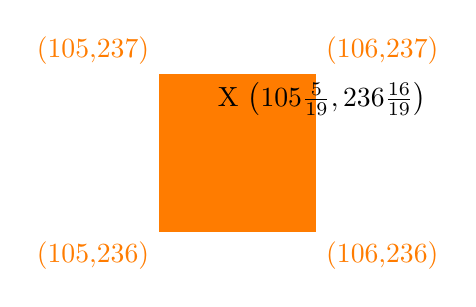
\begin{tikzpicture}[scale=2]
	\fill[color=aa] (0,0) node[anchor=north east] {(105,236)} -- (0,1) node[anchor=south east] {(105,237)} -- (1,1) node[anchor=south west] {(106,237)} -- (1,0) node[anchor=north west] {(106,236)} -- cycle;
	\node[right] at (0.3125,0.842105) {X $\left( 105 \frac{5}{19},236 \frac{16}{19} \right)$};
\end{tikzpicture}

\alert{ This method is not guaranteed to give the optimum solution
(particularly if the objective line is almost parallel to one of the
constraints). However, if more searching is required some direction
should be given in the question.}
	\end{column}
	\end{columns}

	\centering
	\adjustbox{max width=\linewidth}{
		\colorbox{cc!30}{
			\begin{nicetable}{ccccc}
				Point & $5x+2y\geq 1000$ &  $3x+5y \geq 1500$ & In R? &  $C=x+y$ \\ \hline
				(105,236) &  $997 \not\geq 1000$ & & & \\
				(105,237) & $999\not\geq 1000$ & & & \\
				(106,236) &  $1002 \geq 1000$ &  $1498 \not \geq 1500$ & & \\
				(106,237) & $1004\geq 1000$ &  $1503 \geq 1500$ & yes & 343 \\
				\end{nicetable}
	}

	}

	\alert{A common mistake is to forget to check whether the nearby points are in the feasible region.}
\end{frame}

\begin{frame}[shrink=25]{Past Paper Question}
	\begin{columns}
	\begin{column}{.65\linewidth}
	\begin{problem}
		A family business makes and sells two kinds of kitchen table.

		Each pine table takes 6 hours to make and the cost of materials is £30.

		Each oak table takes 10 hours to make and the cost of materials is £70.

		Each month, the business has 360 hours available for making the tables and £2100 available for the materials.

		Each month, the business sells all of its tables to a wholesaler.

		The wholesaler specifies that it requires at least 10 oak tables per month and at least as many pine tables as oak tables.

		Each pine table sold gives the business a profit of £40 and each oak table sold gives the business a profit of £75.

		Use a graphical method to find the number of each type of table the business should make each month, in order to maximise its total profit.

		Show clearly how you obtain your answer.
	\end{problem}
	\end{column}
	\begin{column}{.35\linewidth}
\adjustbox{max width=\linewidth}{
          \begin{tikzpicture}
                  \begin{axis}[mlineplot,width=8cm,height=8cm,
                          xmin= 0, xmax= 80,
                          ymin= 0, ymax = 40,
                          axis lines = middle,
                          xlabel={$x$},
                          ylabel={$y$},
                          ]
                          \addplot[name path=A,color=aa,domain=0:80] {36-0.6*x};
                          \addplot[name path=B,color=aa,domain=0:80] {x};
                          \addplot[color=aa,domain=0:80] {-3*x/7+210/7};
			  \draw[color=aa] (axis cs:0,10) -- (axis cs:80,10);
                  \end{axis}
          \end{tikzpicture}
  }
	
	\end{column}
	\end{columns}

	\begin{columns}
	\begin{column}{.5\linewidth}
		\begin{solution}<2->	
	$x=$ number of pine tables.

	 $y=$ number of oak tables.

	 $30x+70y \leq 2100$

	  $6x+10y \leq 360$

	   $y \leq x, y \geq 10, x \geq 0$ 
   \end{solution}
	\end{column}
	\begin{column}{.5\linewidth}
		\begin{solution}<4->
The objective line has a gradient of $-\frac{8}{15}$. 

35 Pine tables and 15 Oak Tables (Profit=£2525) 

\alert{Make sure you get the marks for defining and state the variables and result in context}
		\end{solution}
	\end{column}
	\end{columns}
\end{frame}


\end{document}
